\documentclass[10pt]{beamer}

\usetheme[progressbar=frametitle]{metropolis}
\usepackage{appendixnumberbeamer}
\usepackage[normalem]{ulem}
\usepackage{booktabs}
\usepackage[scale=2]{ccicons}

\usepackage{pgfplots}
\usepgfplotslibrary{dateplot}

\usepackage{xspace}
\newcommand{\themename}{\textbf{\textsc{metropolis}}\xspace}

\usepackage{tikz}
\title{Can Communication Protocols Find Small LPs?}
\subtitle{Knapsack Cover, Extended Formulations, and Communication Complexity}
% \date{\today}
\date{}
\author{By W. Justin Toth}
\institute{CS860 - Communication Complexity}
\titlegraphic{\hfill
\includegraphics[height=1.5cm]{logo.png}}

\setbeamercolor{alerted text}{fg=blue}

%Macros
\newcommand{\A}{\mathbb{A}} 
\newcommand{\D}{\mathbb{D}} \newcommand{\F}{\mathbb{F}}
\newcommand{\N}{\mathbb{N}} \newcommand{\R}{\mathbb{R}}
 \newcommand{\Z}{\mathbb{Z}}
\newcommand{\Q}{\mathbb{Q}}
 
 
\newcommand{\cA}{\mathcal{A}} \newcommand{\cB}{\mathcal{B}}
\newcommand{\cC}{\mathcal{C}} \newcommand{\cD}{\mathcal{D}}
\newcommand{\cE}{\mathcal{E}} \newcommand{\cF}{\mathcal{F}}
\newcommand{\cG}{\mathcal{G}} \newcommand{\cH}{\mathcal{H}}
\newcommand{\cI}{\mathcal{I}} \newcommand{\cJ}{\mathcal{J}}
\newcommand{\cK}{\mathcal{K}} \newcommand{\cL}{\mathcal{L}}
\newcommand{\cM}{\mathcal{M}} \newcommand{\cN}{\mathcal{N}}
\newcommand{\cO}{\mathcal{O}} \newcommand{\cP}{\mathcal{P}}
\newcommand{\cQ}{\mathcal{Q}} \newcommand{\cR}{\mathcal{R}}
\newcommand{\cS}{\mathcal{S}} \newcommand{\cT}{\mathcal{T}}
\newcommand{\cU}{\mathcal{U}} \newcommand{\cV}{\mathcal{V}}
\newcommand{\cW}{\mathcal{W}} \newcommand{\cX}{\mathcal{X}}
\newcommand{\cY}{\mathcal{Y}} \newcommand{\cZ}{\mathcal{Z}}

\newcommand{\tight}{tight}
\newcommand{\Mtight}{\cM_{\tight}}
\newcommand{\uni}{uni}
\newcommand{\Muni}{\cM_{\uni}}
\newcommand{\core}{\ensuremath{\mbox{core}}}
\DeclareMathOperator{\suppOp}{supp}
\newcommand{\supp}{\suppOp}

\DeclareMathOperator{\convOp}{conv}
\newcommand{\conv}{\convOp}

\newcommand{\level}{\mathrm{lev}}
\newcommand{\set}{\mathrm{set}}
\newcommand{\fix}{\mathrm{Fix}}

\DeclareMathOperator{\exOp}{excess}
\newcommand{\ex}{\exOp}

\DeclareMathOperator{\symOp}{diff}
\newcommand{\sym}{\symOp}

\DeclareMathOperator{\parent}{parent}
\DeclareMathOperator{\optop}{top}
\DeclareMathOperator{\excess}{excess}
\DeclareMathOperator{\opspan}{span}


\begin{document}
\setbeamercolor{background canvas}{bg=white}
\maketitle

\begin{frame}{The Min Knapsack Problem}
Given $n$ items with individual sizes, $s_i$, and costs, $c_i$, for $i \in [n]$.
\vfill
Also given a demand $D$. Want to compute the \alert{Min Knapsack}

\begin{align*}
\min\ &\sum_{i\in [n]} c_i x_i \\
\text{s.t.} &\sum_{i \in [n]} s_i x_i \geq D \\
&x \in \{0,1\}^n.
\end{align*}
\vfill
Standard Linear Programming relaxation has an unbounded integrality gap.
\end{frame}
\begin{frame}{Knapsack Cover Inequalities}
LP relaxation can be strengthened to an integrality gap of $2$ via all Knapsack Cover Inequalities.
\vfill
Knapsack Cover Inequality for $B\subseteq [n]$ is the inequality of the form 
$$\sum_{i \in [n]\backslash B} s_i(B) x_i \geq D(B),$$
where $D(B) = \max\{D-\sum_{i\in B} s_i, 0\}$ and $s_i(B) = \min\{s_i, D(B)\}.$
\vfill
\textbf{Big Open Question:} Is there a polynomial size formulation for Knapsack Cover LP?
\end{frame}
\begin{frame}{Extended Formulations}
    \begin{columns}
        \begin{column}{0.5\textwidth}
    \begin{figure}
        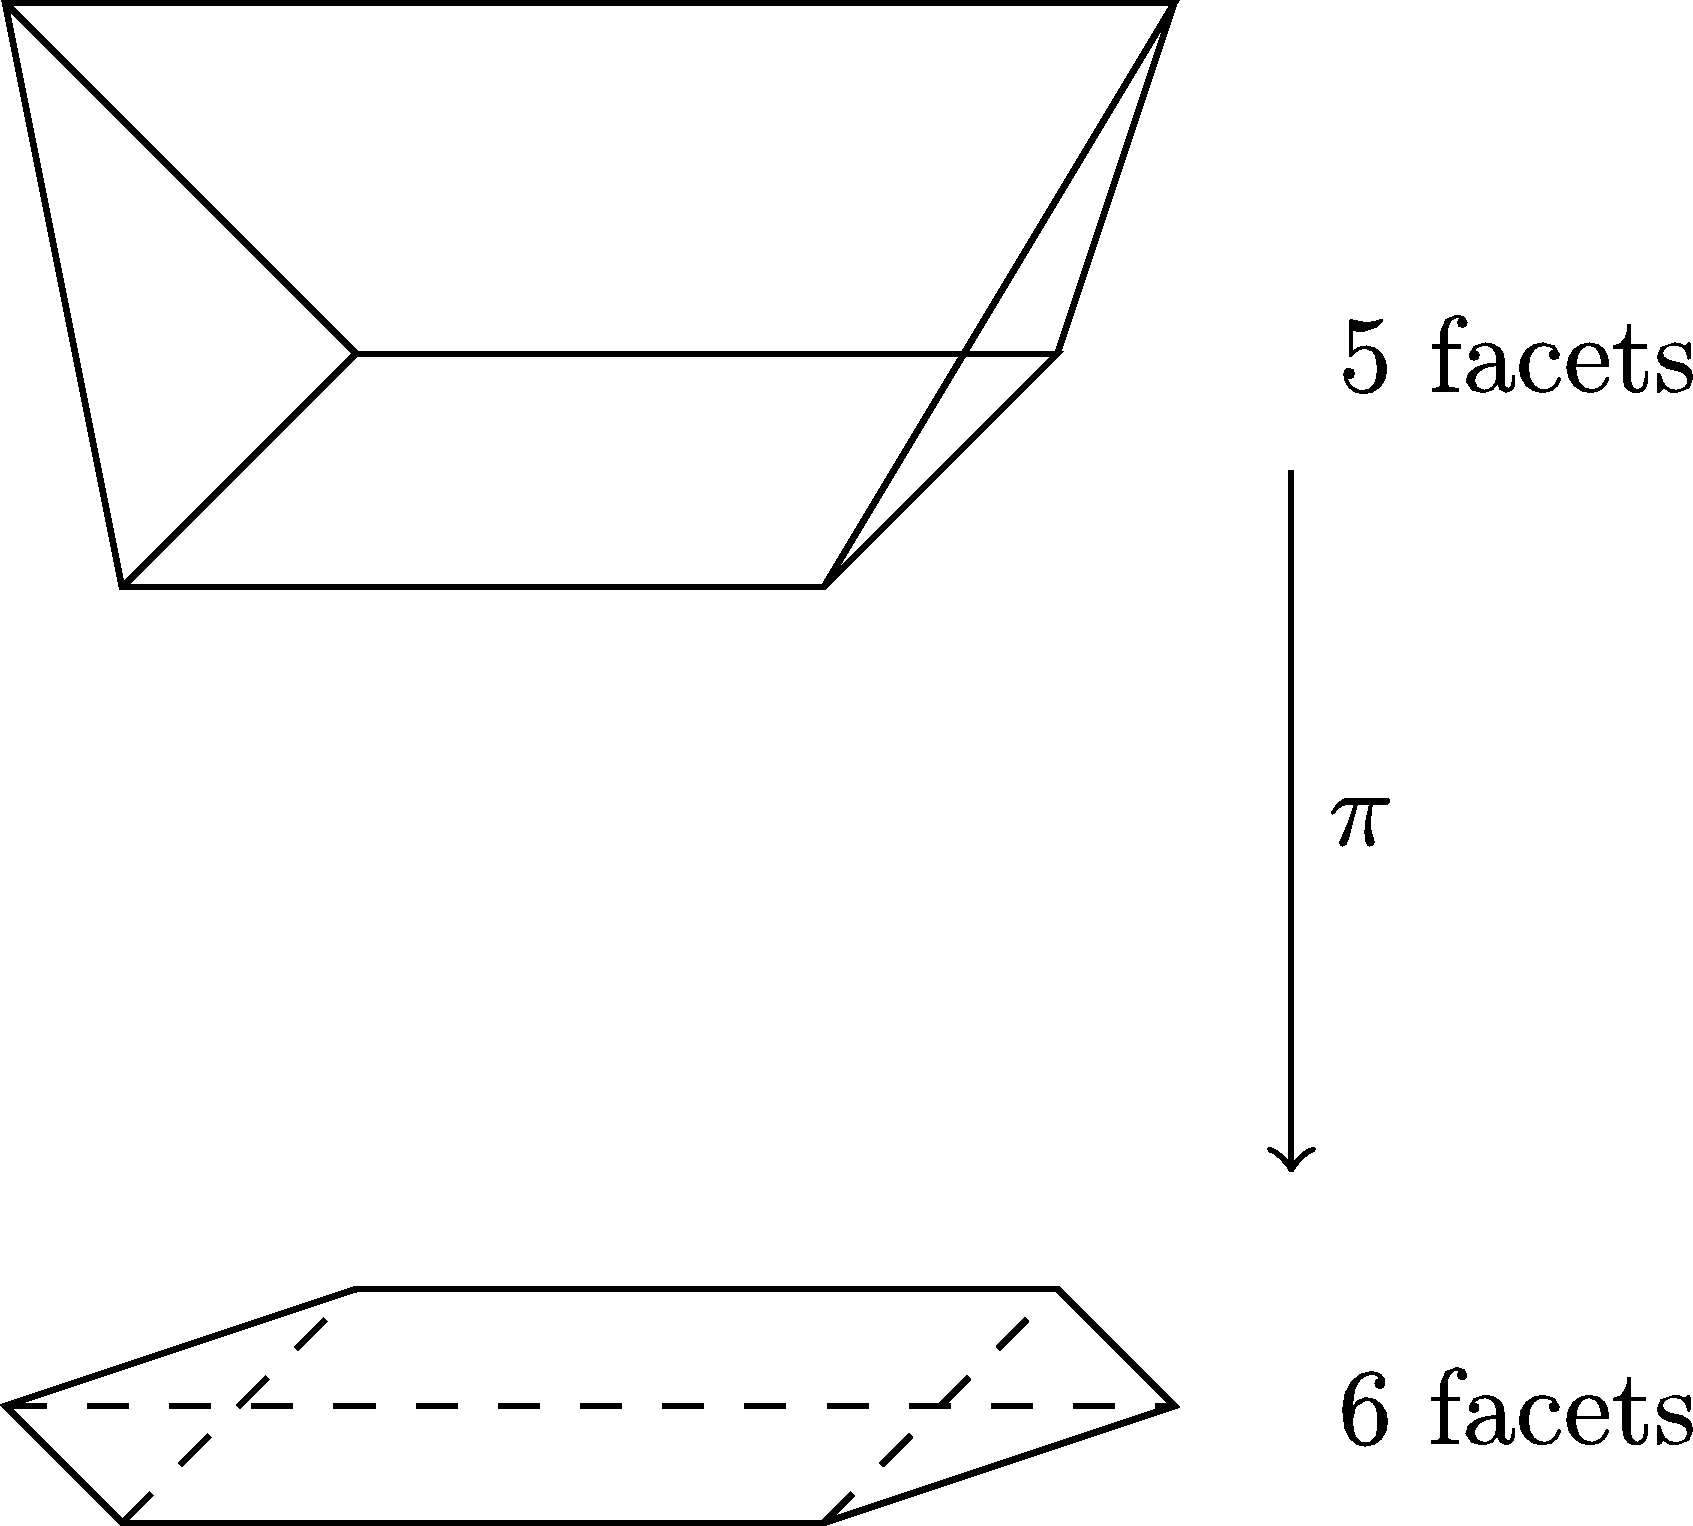
\includegraphics[scale=0.075]{std_ex.png}
    \end{figure}
\end{column}
\begin{column}{0.5\textwidth}
\textbf{Extension Complexity:} Min number of facets to describe a polytope as the projection of a higher dimensional polyhedron.
\end{column}
\end{columns}
\end{frame}
\begin{frame}{Communication Protocols for the Slack Matrix}
\end{frame}
\begin{frame}{Results}
\end{frame}
\end{document}
